\begin{frame}{Framework with Plug-Ins}
	\begin{mycolumns}[widths={50,50},animation=none]
		\mydefinition{Framework and Hot Spot}{
			A framework is a set of classes that embodies an abstract design for solutions to a family of related problems, and supports reuse at a larger granularity than classes. A framework is open for extension at explicit hot spots.				
		}
		\mydefinition{Plug-In}{
			A plug-in extends hot spots of a [...] framework with custom behavior. A plug-in can be separately compiled and deployed.	
		}
		\mynote{}{
			Frameworks with plug-ins are also called blackbox frameworks: Developers need to understand interfaces, but not the internal framework implementation.
		}
	\mynextcolumn
		TODO: links cites
		TODO: rechts Inversion of Control
		Hollywood principle: ``Don’t call us, we’ll call you''
		
		\pic[width=0.5\linewidth]{library_vs_framework}
		
		\mynote{}{
			\begin{itemize}
				\item Can be understood in terms of the observer and/or strategy pattern: The framework exposes explicit hot spots, at which plug-ins can register observers and strategies.
				\item Requires preplanning for possible future extensions
			\end{itemize}
		}		
	\end{mycolumns}
\end{frame}



\begin{frame}{Preplanned Bike Extensions}
	\begin{mycolumns}[columns=4,T]
		\centering\pic[width=\linewidth]{bike-extensionpoint1}

		bike lock
	\mynextcolumn
		\centering\pic[width=\linewidth]{bike-extensionpoint2}

		front wheel brake
	\mynextcolumn
		\centering\pic[width=\linewidth]{bike-extensionpoint3}

		rear wheel brake
	\mynextcolumn
		\centering\pic[width=\linewidth]{bike-extensionpoint4}

		kickstand
	\end{mycolumns}
\end{frame}

\begin{frame}{Preplanned Bike Extensions}
	\begin{mycolumns}[columns=5,widths={30,5,30,5,30}]
		\centering\pic[width=\linewidth]{bike-extensionpoint1-withoutplugin}

		framework with extension~points
	\mynextcolumn
		\centering\Huge +
	\mynextcolumn
		\centering\pic[width=\linewidth]{bike-lock}

		plug-ins\\~
	\mynextcolumn
		\centering\Huge =
	\mynextcolumn
		\centering\pic[width=\linewidth]{bike-extensionpoint1}

		framework with plug-ins\\~
	\end{mycolumns}
\end{frame}


\begin{frame}{Simple Example: A Family of Dialogs}
	\begin{itemize}
		\item Familie von Dialogen, bestehend aus Textfeld und Button\\
		\pic{dialog1}
		\pic{dialog2}
		\pic{dialog3}
		\item 90\% des Quelltexts sind gleich
		\begin{itemize}
			\item Main Methode
			\item Initialisierung von Fenstern, Textfeld und Button
			\item Layout
			\item Schließen des Fensters
			\item \ldots
		\end{itemize}
	\end{itemize}
\end{frame}


\begin{frame}[fragile]{Simple Example: A Family of Dialogs}
	\small\begin{mycolumns}[columns=2,widths={50,50}]
\begin{codetight}{}
public class Calc extends JFrame {
	private JTextField textfield;
	public static void main(String[] args) {
		new Calc().setVisible(true);
	}
	public Calc() { init(); }
	protected void init() {
		JPanel p = new JPanel(new BorderLayout());
		p.setBorder(new BevelBorder(/* ... */));
		JButton button = new JButton();
		button.setText(@"calculate"@);
		p.add(button, BorderLayout.EAST);
		textfield = new JTextField("");
		textfield.setText(@"10 / 2 + 6"@);
		textfield.setPreferredSize(new Dimension(350, 40));
		p.add(textfield, BorderLayout.WEST);
		button.addActionListener(new ActionListener() 
			{ @/* calculate */@ });
		this.setp(p);
		this.pack();
		this.setTitle(@"My Great Calculator"@);
		// ...
	}
}
\end{codetight}
		\mynextcolumn
\begin{codetight}{}
public class Ping extends JFrame {
	private JTextField textfield;
	public static void main(String[] args) {
		new Calc().setVisible(true);
	}
	public Calc() { init(); }
	protected void init() {
		JPanel p = new JPanel(new BorderLayout());
		p.setBorder(new BevelBorder(/* ... */));
		JButton button = new JButton();
		button.setText(@"ping"@);
		p.add(button, BorderLayout.EAST);
		textfield = new JTextField("");
		textfield.setText(@"127.0.0.1"@);
		textfield.setPreferredSize(new Dimension(350, 40));
		p.add(textfield, BorderLayout.WEST);
		button.addActionListener(new ActionListener() 
			{ @/* calculate */@ });
		this.setp(p);
		this.pack();	
		this.setTitle(@"Ping"@);
		// ...
	}
}
\end{codetight}
	\end{mycolumns}
\end{frame}


\begin{frame}[fragile]{Simple Example: A Family of Dialogs}
	\tiny\begin{mycolumns}[columns=2,widths={50,50}]
\begin{codetight}{}
public class Application extends JFrame {
	private JTextField textfield;
	private Plugin plugin;

	public Application(Plugin plugin) {
		this.plugin = plugin;
		plugin.setApplication(this);
		init();
	}

	protected void init() {
		JPanel p = new JPanel(new BorderLayout());
		p.setBorder(new BevelBorder(/*...*/);
		JButton button = new JButton();
		button.setText(plugin.getButtonText());
		p.add(button, BorderLayout.EAST);
		textfield = new JTextField("");
		textfield.setText(plugin.getInititalText());
		textfield.setPreferredSize(new Dimension(200, 20));
		p.add(textfield, BorderLayout.WEST);		
		button.addActionListener(/* . . . plugin.buttonClicked(); . . . */);
		this.setContentPane(p);
		// ...
	}

	public String getInput() {
		return textfield.getText();
	}
}
\end{codetight}
		\mynextcolumn
\begin{codetight}{}
public interface Plugin {
	String getApplicationTitle();
	String getButtonText();
	String getInititalText();
	void buttonClicked();
	void setApplication(Application app);
}
\end{codetight}
\begin{codetight}{}
public class CalcPlugin implements Plugin {
	private Application application;

	public String getApplicationTitle() {
		return "My Great Calculator";
	}
	public String getButtonText() {
		return "calculate";
	}
	public String getInititalText() {
		return "10 / 2 + 6";
	}
	public void buttonClicked() {
		calculate(application.getInput());
	}
	public void setApplication(Application app) {
		application = app;
	}
	private void calculate(String expression) {
		/* calculate */
	}
}
\end{codetight}
	\end{mycolumns}
\end{frame}

\begin{frame}[fragile]{Simple Example: A Family of Dialogs}
	\tiny\begin{mycolumns}[columns=2,widths={50,50}]
\begin{codetight}{}
public class Application extends JFrame @implements InputProvider@ {
	private JTextField textfield;
	private Plugin plugin;

	public Application(Plugin plugin) {
		this.plugin = plugin;
		@plugin.setInputProvider(this);@
		init();
	}

	protected void init() {
		JPanel p = new JPanel(new BorderLayout());
		p.setBorder(new BevelBorder(/*...*/);
		JButton button = new JButton();
		button.setText(plugin.getButtonText());
		p.add(button, BorderLayout.EAST);
		textfield = new JTextField("");
		textfield.setText(plugin.getInititalText());
		textfield.setPreferredSize(new Dimension(200, 20));
		p.add(textfield, BorderLayout.WEST);		
		button.addActionListener(/* . . . plugin.buttonClicked(); . . . */);
		this.setContentPane(p);
		// ...
	}

	public String getInput() {
		return textfield.getText();
	}
}
\end{codetight}
		\mynextcolumn
\begin{codetight}{}
public interface InputProvider {
	public String getInput();
}
\end{codetight}
\begin{codetight}{}
public interface Plugin {
	String getApplicationTitle();
	String getButtonText();
	String getInititalText();
	void buttonClicked();
	@void setInputProvider(InputProvider p);@
}
\end{codetight}
\begin{codetight}{}
public class CalcPlugin implements Plugin {
	@private InputProvider inputProvider;@

	public String getApplicationTitle() {
		return "My Great Calculator";
	}
	public String getButtonText() {
		return "calculate";
	}
	public String getInititalText() {
		return "10 / 2 + 6";
	}
	public void buttonClicked() {
		calculate(@inputProvider.getInput()@);
	}
	@public void setInputProvider(InputProvider p) {
		inputProvider = p;
	}@
	private void calculate(String expression) {
		/* calculate */
	}
}
\end{codetight}
	\end{mycolumns}
\end{frame}

\begin{frame}{Plug-In Loading and Management}
	\begin{mycolumns}[widths={50,50},animation=none]
		\mynote{Simple example vs.\ reality}{
			Simplification in our previous example:
			\begin{itemize}
				\item A single extension point supporting the registration of a single plug-in 
				\item Plug-in implementation known at compile-time 
			\end{itemize}
			Typical requirements in practice:
			\begin{itemize}
				\item Many extension points supporting the registration of arbitrarily many plug-ins 
				\item Plug-in implementation provided by third parties (requires load-time variability)
			\end{itemize}
		}		
	\mynextcolumn
		\mydefinition{Plug-in Loader}{
			\begin{itemize}
				\item Searches in a dedicated directory for DLL/Jar/XML files
				\item Tests whether file implements a plug-in
				\item Checks dependencies
				\item Initializes plug-ins
			\end{itemize}
		}
		\mydefinition{Plug-In Manager}{
			\begin{itemize}
				\item GUI and/or console interface for plug-in administration and configuration.
			\end{itemize}
		}
	\end{mycolumns}
\end{frame}

\begin{frame}[fragile]{Example: Plug-In Loading and Management}
	\tiny\begin{mycolumns}[columns=2,widths={50,50}]
\begin{codetight}{Plug-In Loader using Java Reflection}
public class Starter {
	public static void main(String[] args) {
		if (args.length != 1)
			System.out.println("Plugin name not specified");
		else {
			String pluginName = args[0];
			try {
				Class pluginClass = Class.forName(pluginName);
				new Application((Plugin) pluginClass.newInstance()).setVisible(true);
			} catch (Exception e) {
				System.out.println("Cannot load plugin " + pluginName + ", reason: " + e);
			}
		}
	}
}
\end{codetight}
		\mynextcolumn
\begin{codetight}{Handling multiple Plug-Ins}
public class Application {
	private List<Plugin> plugins;

	public Application(List<Plugin> plugins) {
		this.plugins = plugins;
		for (Plugin plugin : plugins) {
			plugin.init();
		}
	}

	public Message processMsg(Message msg) {
		for (Plugin plugin : plugins) {
			msg = plugin.process(msg);
			// ...
		}
		return msg;
	}
}
\end{codetight}
	\end{mycolumns}
\end{frame}

\begin{frame}{Frameworks in the Wild: Eclipse}
	\begin{mycolumns}[widths={70,30},animation=none]
		\pic[width=\linewidth]{eclipse_overview}
	\mynextcolumn
		\myexample{Versatile IDE}{
			\begin{itemize}
				\item Lots of common functionality required by any IDE
					(e.g., editors, incremental project build, etc.) 
				\item Only language-specific extensions need to be registered
					(e.g., syntax highlighting, compiler, etc.)
			\end{itemize}
		}
		\mynote{Specifically in Eclipse}{
			\begin{itemize}
				\item Actually a set of (recursively nested) frameworks
				\item Largely declarative description of extension points
			\end{itemize}
		}
	\end{mycolumns}
\end{frame}

\begin{frame}{Frameworks in the Wild: Eclipse \mytitlesource{\featureide}}
	\leftorright{
		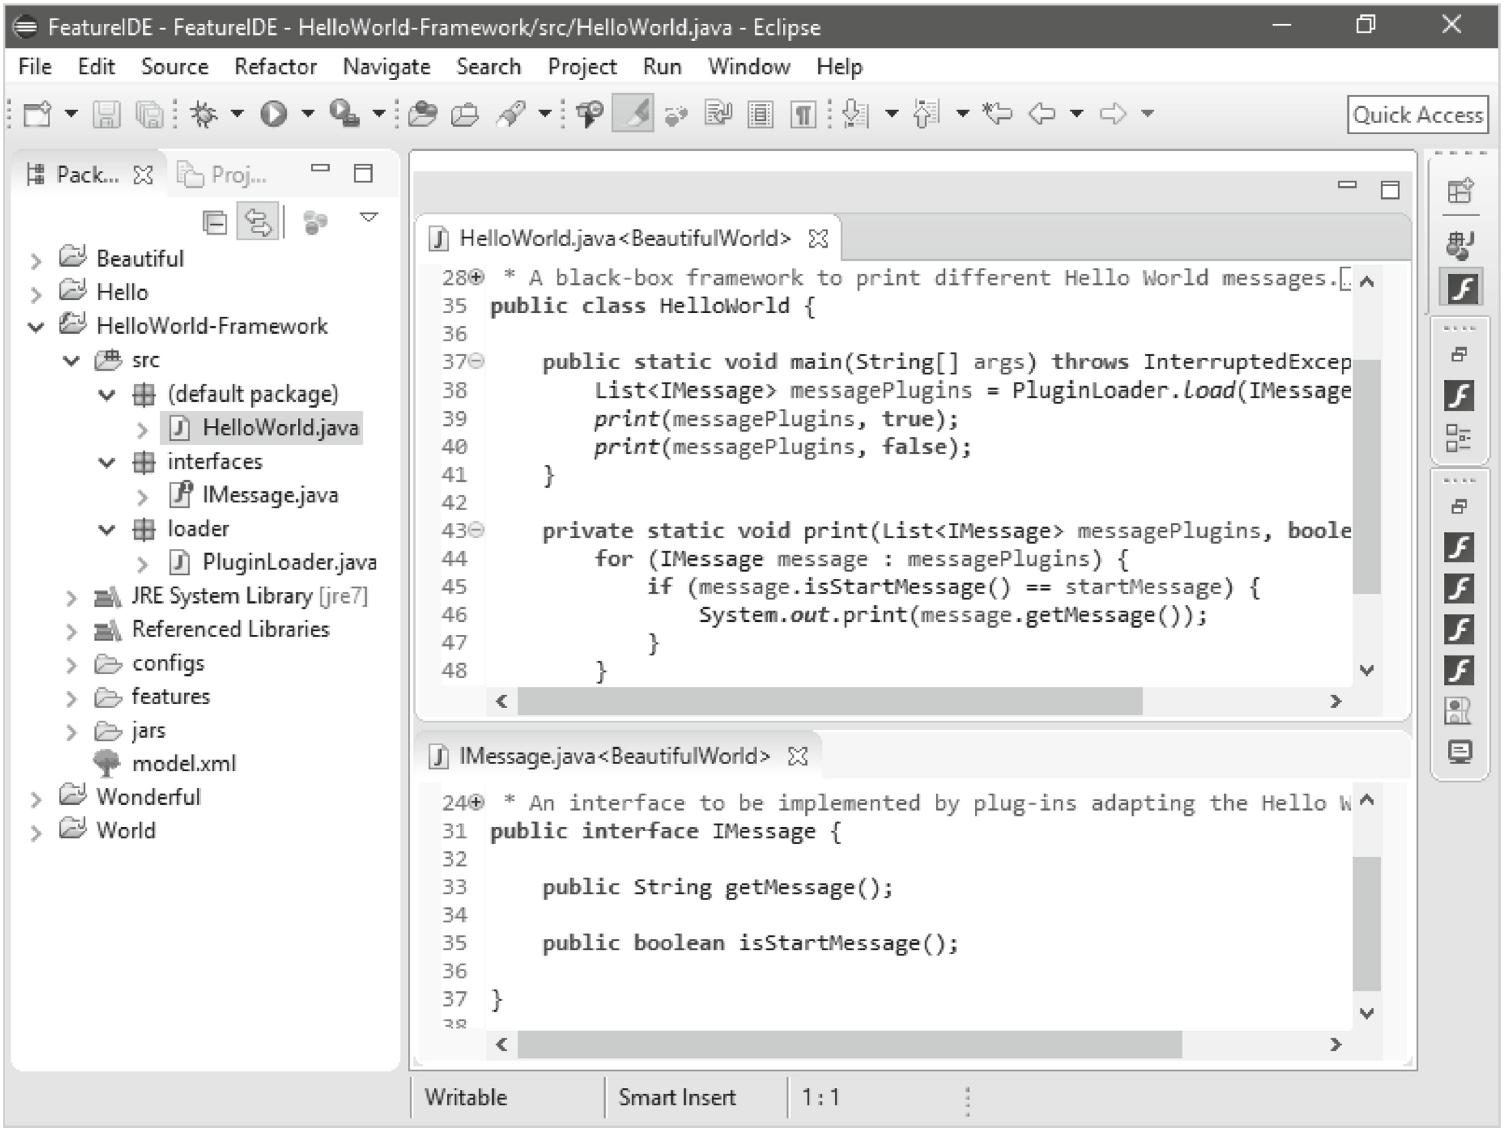
\includegraphics[width=\linewidth]{framework-with-plugins}
	}{
		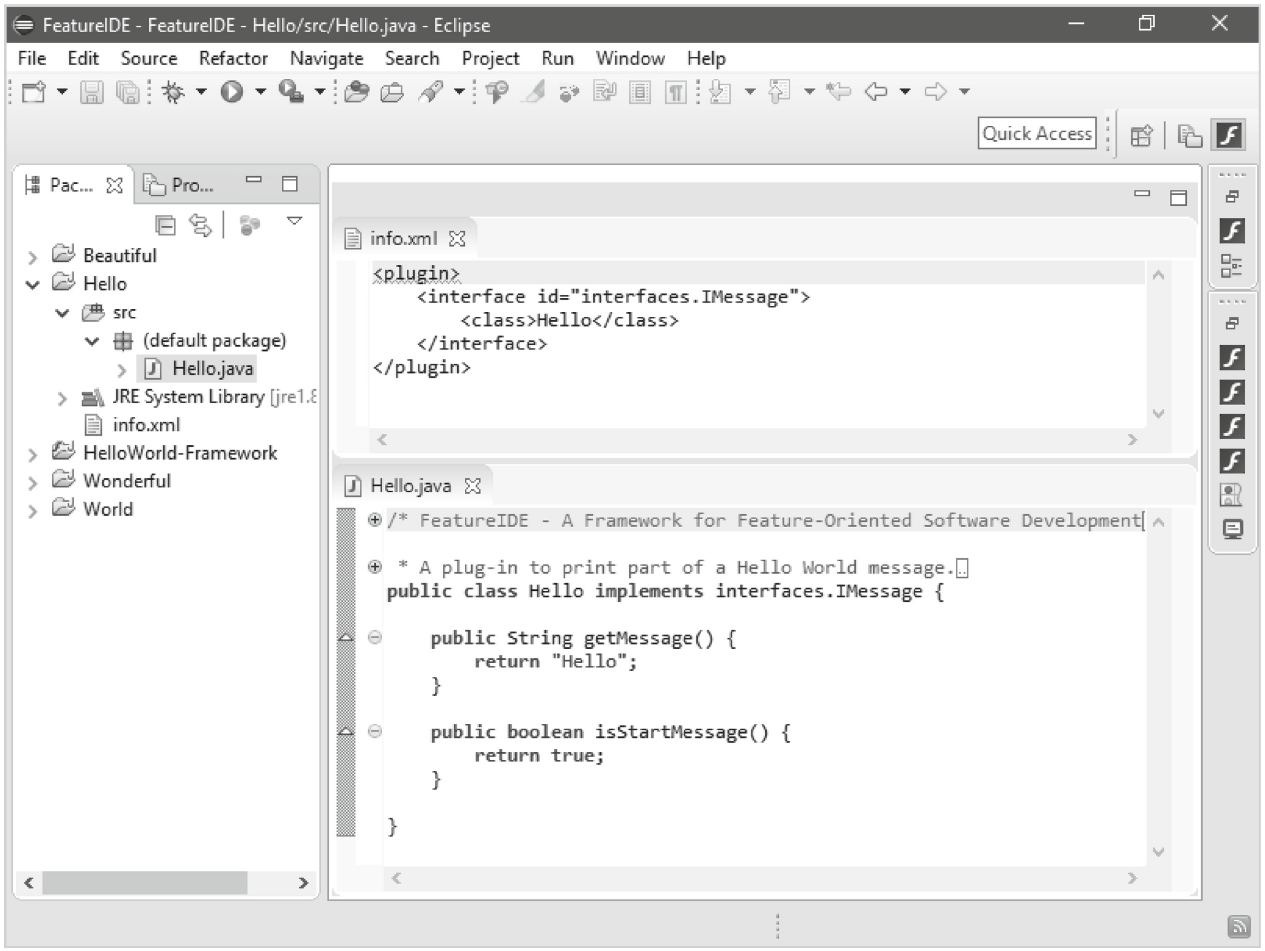
\includegraphics[width=\linewidth]{framework-a-plugin}
	}
\end{frame}

\begin{frame}{Frameworks in the Wild: Further Examples}
	\begin{mycolumns}[widths={60,40},animation=none]
		\myexample{}{
			\begin{itemize}
				\item Other IDEs (e.g. IntelliJ, ...)
				\item Frontend frameworks (e.g., MacApp, Swing, SWT, MFC, ...)
				\item Backend frameworks (e.g., Spring Boot, Ruby on Rails, Django, ...) 
				\item Multimedia frameworks (e.g., DirectX, ...)
				\item Raster/vector graphics editors (e.g., Adobe Photoshop, MS Visio, ...)
				\item Instant messenger framewoks (z.B. Miranda, Trillian)
				\item Compiler frameworks (z.B. Polyglot, abc, JustAddJ)
				\item Web browsers (e.g., Firefox, ...)
				\item E-Mail clients (e.g., Thunderbird, ...)
				\item etc.
			\end{itemize}
		}		
	\mynextcolumn
		... TODO logos
	\end{mycolumns}
\end{frame}


\begin{frame}{Framework-Based Implementation of Software Product Lines}
	\begin{mycolumns}[widths={40,60},animation=none]
		\myexample{Recap: Service-Based Implementation}{
			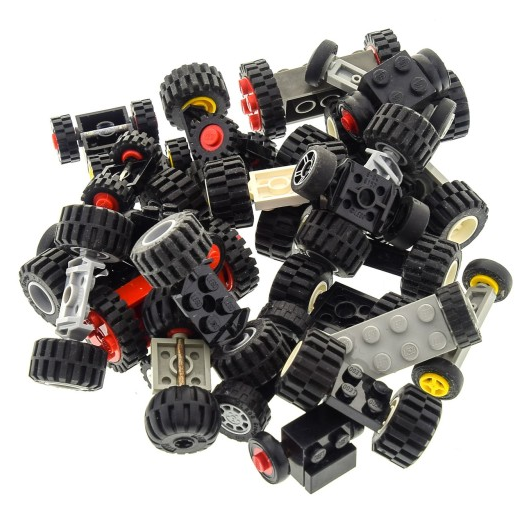
\includegraphics[width=.23\linewidth,height=1.0cm]{lego_components} 
				\vspace*{\fill}
					$+$ 
				\vspace*{\fill}	
			
\includegraphics[width=.23\linewidth,height=1.0cm]{lego_orchestration}
				\vspace*{\fill}
					$=$ 
				\vspace*{\fill}	
			
\includegraphics[width=.3\linewidth,height=1.0cm]{lego_product}
		}		
		\myexample{Still needs some specification for ``composition''}{
			\centering
			
\includegraphics[width=.65\linewidth,height=2.5cm]{lego_orchestration}				
		}				
	\mynextcolumn
		\mydefinition{Same Idea}{
			\begin{itemize}
				\item Features are implemented by different plug-ins
				\item Feature selection determines the plug-ins to be loaded and registered 
			\end{itemize}
		}	
		\mynote{}{
			Neither individual glue code nor specification of service composition required.
		}	
		\myexample{}{
			TODO: Erstes Bild ohne Räder
			
\includegraphics[width=.27\linewidth,height=1.75cm]{lego_product} 
				\vspace*{\fill}
					$+$ 
				\vspace*{\fill}	
			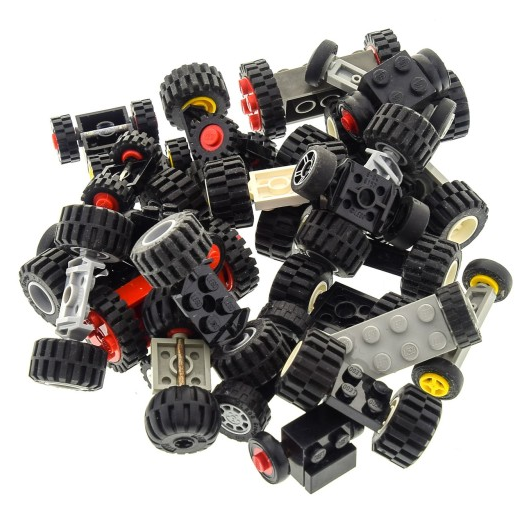
\includegraphics[width=.27\linewidth,height=1.75cm]{lego_components}
				\vspace*{\fill}
					$=$ 
				\vspace*{\fill}	
			
\includegraphics[width=.35\linewidth,height=1.75cm]{lego_product}
		}	
		\mynote{}{
			Potential for full automation comes at a price: The preplanning problem (see next slides).
		}
	\end{mycolumns}	
\end{frame}

\begin{frame}[fragile]{Example: Extending Basic Graphs by Plug-Ins?}
	\tiny\begin{mycolumns}[columns=2,widths={50,50}]
\begin{codetight}{}
public class Graph {
	// ...
	private List<Node> nodes = new ArrayList<Node>();	
	private List<GraphPlugin> plugins = new ArrayList<GraphPlugin>();
	
	public void registerPlugin(GraphPlugin p){
		plugins.add(p);
	}
	
	public void addNode(int id, Color c){
		Node n = new Node(id);
		notifyAdd(n, c);
		nodes.add(n);
	}
	
	public void print() {
		for (Node n : nodes) {
			notifyPrint(n);
			// ...
		}
		// ...
	}
	
	private void notifyAdd(Node n, Color c) {
		for (GraphPlugin p : plugins) {
			p.aboutToAdd(n, c);
		}
	}
	
	private void notifyPrint(Node n) {
		for (GraphPlugin p : plugins) {
			p.aboutToPrint(n);
		}
	}
	// ...
}
\end{codetight}
		\mynextcolumn
\begin{codetight}{}
public interface GraphPlugin {
	public void aboutToAdd(Node n, Color c);
	public void aboutToAdd(Edge e, Weight w);
	public void aboutToPrint(Node n);
	public void aboutToPrint(Edge e);
}
\end{codetight}
\begin{codetight}{}
public class ColorPlugin implements GraphPlugin {
	private Map<Node, Color> map = new HashMap<Node, Color>();

	public void aboutToAdd(Node n, Color c) {
		map.put(n, c);
	}
	public void aboutToAdd(Edge e, Weight w) {
		// do nothing
	}
	public void aboutToPrint(Node n) {
		Color c = map.get(n);
		Color.setDisplayColor(c);
	}
	public void aboutToPrint(Edge e) {
		// do nothing
	}
}
\end{codetight}
	\end{mycolumns}
\end{frame}

\begin{frame}{Challenges and Problems }
	\begin{mycolumns}[widths={50,50},animation=none]
		\myexample{}{
			In our example, we can observe that:
			\begin{itemize}
				\item There are lots of empty methods in the ColorPlugin 
				\item The Framework consults all registered plug-ins before printing a node or edge
			\end{itemize}
		}		
		\mydefinition{General Challenge: Cross-cutting Concerns}{
			Implementing cross-cutting concerns as plug-ins 
			\begin{itemize}				
				\item typically leads to huge interfaces, large parts of which are irrelevant for a dedicated plug-in 
				\item causes lots of communication overhead between plug-ins and framework
			\end{itemize}
		}
	\mynextcolumn
		\myexample{}{
			If we were not familiar with our graph library, would we anticipate that:
			\begin{itemize}
				\item Colors and weights should be part of the Plugin interface?
				\item Every plug-in needs to be notified that the framework is about to print a node or edge? 
			\end{itemize}
		}
		\mydefinition{Generally known as Preplanning Problem}{
			\begin{itemize}
				\item Hard to identify and foresee the relevant hot spots and nature of extensions
				\item Developing a framework needs lots of expertise and excellent domain knowledge 
			\end{itemize}
		}	
	\end{mycolumns}
\end{frame}
